% ============================================================
%  R. Nielsen, "Philosophie og Mathematik. En propædeutisk Afhandling."
%  Kjøbenhavn: Forlagt af den Gyldendalske Boghandling (F. Hegel);
%  Thieles Bogtrykkeri, 1857.
%  TRANSCRIPTION (Danish) — from the Kongelige Bibliotek (KB) DOD scan.
%
%  Scan: ~/bibliotek/Nielsen, Rasmus/1857phil-math.pdf
%        KB "Digitalisering on Demand" scan (NOT Google Books). 93 PDF pp.;
%        KB pp. 1--5 = DOD cover + boilerplate; body = printed pp. 1--84 ("84 s.").
%        (The other file, Philosophie_og_Mathematik.pdf, 88 pp, IS the lower-
%        quality Google Books scan — do not use it.)
%  TYPE: Fraktur (Danish body); Greek/Latin technical terms in antiqua.
%        OCR with the tessdata_best `Fraktur` script model (NOT -l dan),
%        then image-verify every page (letterspacing -> \emph{}, every
%        equation and figure cropped and zoomed).
%
%  OFFSET (VERIFIED at 3 points): PDF = printed + 5.
%        PDF 10 = printed 5;  PDF 20 = printed 15;  PDF 30 = printed 25.
%        Title page = PDF 6 (printed 1); blank verso = PDF 7 (printed 2);
%        body text begins PDF 8 = printed 3 (drop-cap "Nærværende
%        Afhandlings Forfatter ..."). No Forord / Indhold / Indledning:
%        the essay opens directly with the text.
%
%  MATH + FIGURES: math-heavy (functions, fractions, roots, sub/superscripts)
%        + geometric diagrams (asymptote/hyperbola on printed p.25, etc.).
%        FIGURE POLICY (agreed with Hans): redraw every figure in TikZ,
%        image-verified against the scan. Hence \usepackage{tikz}.
%
%  STATUS: IN PROGRESS. Done: preamble + title page (front matter).
%        Body not yet begun. Resume at printed p.3 (PDF 8). See RESUME-NOTES.md.
% ============================================================
\documentclass[12pt]{book}
\usepackage[utf8]{inputenc}
\usepackage[T1]{fontenc}
\usepackage[danish]{babel}
\usepackage[protrusion=true,expansion=true]{microtype}
\usepackage[margin=1.4in]{geometry}
\usepackage{setspace}
\usepackage{amsmath}
\usepackage{graphicx}
\usepackage{tikz}
\usetikzlibrary{calc,intersections,arrows.meta}
\usepackage{libertinus}
\usepackage{libertinust1math}
\usepackage{textalpha}   % polytonic Greek typed directly
\usepackage{fancyhdr}
\usepackage[colorlinks=true,linkcolor=black,urlcolor=black,
  pdftitle={Philosophie og Mathematik},
  pdfauthor={Rasmus Nielsen}]{hyperref}
\setlength{\headheight}{15pt}
\pagestyle{fancy}
\fancyhf{}
\fancyhead[LE,RO]{\thepage}
\fancyhead[RE]{\textit{Philosophie og Mathematik}}
\fancyhead[LO]{\textit{\leftmark}}
\setlength{\parindent}{1.5em}
\setlength{\parskip}{0pt}
\onehalfspacing

\begin{document}

% ============================================================
% TITLE PAGE — PDF 6 (printed p.1)
% ============================================================
\begin{titlepage}
\centering
\vspace*{2cm}
{\Huge\bfseries Philosophie og Mathematik.\par}
\vspace{1.2cm}
\rule{4cm}{0.4pt}\par
\vspace{1.2cm}
{\LARGE En propædeutisk Afhandling\par}
\vspace{0.5cm}
{\large af\par}
\vspace{0.8cm}
{\LARGE\bfseries R.\ Nielsen,\par}
\vspace{0.2cm}
{\normalsize Professor i Philosophien.\par}
\vspace{2.4cm}
\rule{4cm}{0.4pt}\par
\vspace{1.6cm}
{\large\bfseries Kjøbenhavn.\par}
\vspace{0.4cm}
{\normalsize Forlagt af den Gyldendalske Boghandling (F.\ Hegel).\par}
\vspace{0.3cm}
{\small\emph{Thieles Bogtrykkeri.}\par}
\vspace{0.6cm}
{\large 1857.\par}
\end{titlepage}

\frontmatter
\tableofcontents
\mainmatter

% ============================================================
% BODY BEGINS — printed p.3 (PDF 8)
% ============================================================

% ---- printed p.3 (PDF 8): opening statement (stands alone on the page) ----
\noindent Nærværende Afhandlings Forfatter, som hverken er eller vil være
Mathematiker, har i Philosophien, den almindelige Videnskabslære, fundet
Opfordring til at lære ogsaa Mathematikens Sprog, og med Hensyn paa de ledende
Grundbegreber, saavidt muligt, sætte sig ind i dens Tankegang.

% ---- printed p.4 (PDF 9): "Rettelse." (errata). Original page (letterspaced
%      heading) reads only:
%        S. 25, Linie 9: Tilnærmelse til et Uopnaaeligt; læs: Tilnærmelse til
%        et Opnaaeligt.
%      Per repo convention the errata page is NOT reproduced as body text;
%      the correction is APPLIED when p.25 is transcribed (batch 3): the text
%      there must read "Tilnærmelse til et Opnaaeligt".

% ============================================================
% ---- printed p.5 (PDF 10) ----
\begin{center}
  {\large\bfseries I.}\par\vspace{4pt}
  {\Large\bfseries Mathematiske Functioner.}\par\vspace{4pt}
  \rule{2.5cm}{0.4pt}
\end{center}
\addcontentsline{toc}{section}{I.\quad Mathematiske Functioner}
\markboth{Mathematiske Functioner}{Mathematiske Functioner}

\noindent Ordet „Function“ forekommer i meget omfattende Betydning. Hvor der
kan være Tale om Virken, Liden, Handlen, betegner Function en særegen
lovbestemt Virksomhed. Det hedder om en Embedsmand\footnote{Med kategorisk
Eftertryk betoner Kammerherre Norden i „Gamle Minder“ sin „Functionstid“.}, at
han er i Function; man taler om Øiets Function, om en Nerves Function o.\ s.\ v.

Paa de rene Størrelsers Omraade kan der, hvad disse angaaer, dog ligesaalidt
være Tale om egentlig Handlen, som om egentlig Liden: et $a$ kan ikke handle,
et $b$ ikke lide, et $x$ ikke fungere i Lighed enten med en Embedsmand eller en
Nerve.

Da nu alligevel Benævnelsen: „Function“ ikke alene er bibeholdt, men endog som
Begreb fastholdt i Mathematiken, maa man i den mathematiske Anvendelse kunne
paavise noget til Grundbetydningen Svarende.

Vistnok kunne de rene Størrelser ikke udøve reel Virksomhed, men ved at
anbringes i forskjellig Sammenhæng kunne de dog væsentlig forandre de indbyrdes
Forhold. En Størrelse kan, saa at sige, ansættes til forskjellige Bestillinger,
kan som Addend $(a+x)$, som Factor $(ax)$, som Potensexponent $(a^{x},\ x^{a})$,
som Logarithme o.\ s.\ v. erholde en
% ---- printed p.6 (PDF 11) ----
meget forskjellig Indflydelse, og forsaavidt optræde i forskjellige Functioner.

Her er imidlertid en anden Side af Begrebet, som især maa fremhæves i
Størrelseslæren. Man taler ikke blot om at fungere, at være i Function; man
taler ogsaa om det, som tilveiebringes ved den fungerende Virksomhed. Udenfor
Mathematiken tænker man ved Function især paa Virksomheden, i Mathematiken især
paa Resultatet; udenfor Mathematiken gjælder det at være i Function ved Noget,
indenfor Mathematiken at være en Function af Noget. Det lovbundne Forhold
imellem et Afhængigt og et Uafhængigt viser sig imidlertid paa begge Sider.

„Afhænger en Størrelse: $y$, ifølge en vis Lov af andre Størrelser: $x$, $z$,
$t$, $u\ldots$, saa at enhver Værdi af $y$ bestemmes ved de Værdier, som
vilkaarligen tillægges $x$, $z$, $t$, $u\ldots$, siges $y$ at være en Function
af disse Størrelser, alle betragtede som variable, $y$ afhængig, de andre
uafhængige. Dette betegnes almindeligen: $y = f(x,z,t,u\ldots)$“\footnote{C.\
Ramus. Algebra og Functionslære. Kjøbenhavn 1840, S.\ 14.}.

Ifølge denne mathematiske Begrebsbestemmelse ville altsaa Forandringer udgaae
fra de Uafhængige, og udøve deres lovlige Indflydelse paa den Afhængige. For at
minde om Ligheden imellem ikke-mathematiske og mathematiske Functioner, kunde
man da gjerne betragte de Uafhængige: $x$, $z$, $t$, $u\ldots$ som de
Fungerende, de Handlende, der foraarsage Forandringerne i det lidende $y$. Men
da Opfatningen er billedlig, indsees tillige, hvorfor $x$, $z$, $t$, $u\ldots$
ikke siges at være i Function med Hensyn til $y$, medens derimod $y$
udtrykkelig siges at være en Function af $x$, $z$, $t$, $u\ldots$

I Functionen ere altsaa Størrelserne foranderlige; men Størrelser kunne jo
ogsaa være uforanderlige. At enhver Størrelse maa være sig selv lig, og at
enhver Størrelse kan ved Forøgelse eller Formindskelse i hvert Øieblik blive
% ---- printed p.7 (PDF 12) ----
sig selv ulig, er en Modsigelse, der løses i Functionsbegrebet. I og for sig er
ingen Størrelse enten uforanderlig eller foranderlig, thi ingen Størrelse er
Noget alene i og for sig. Om den særegne Størrelse derimod i sit Forhold til
andre Størrelser skal spille den Uforanderliges eller Foranderliges, og, i
Foranderligheden, da igjen den Afhængiges eller den Uafhængiges Rolle,
bestemmes ved Functionen, og bestemmer igjen Functionen.

Er Begrebet: Function, nu for det Første bestemt ved Begrebet Afhængighed, saa
kommer det igjen an paa at bestemme Afhængighedsmaaden, det vil sige: at paavise
Loven.

I den mathematiske Fremstilling af de forskjellige Functioner viser sig en
Skala af Tilfælde, Regel og Lov, som maa blive Gjenstand for Philosophiens
Opmærksomhed.
\[
\begin{aligned}
&\text{At }\ 2(3+4) = 2\cdot 3 + 2\cdot 4 = 6+8 = 2\cdot 7 = 14,\\
&\text{at }\ (3\cdot 4)^{2} = 12^{2} = 3^{2}\cdot 4^{2} = 9\cdot 16 = 144,\\
&\text{at }\ 2^{3}\cdot 2^{4} = (2\cdot 2\cdot 2)\cdot(2\cdot 2\cdot 2\cdot 2)
      = 2^{3+4} = 2^{7},
\end{aligned}
\]
kan erfares ved Forsøg, og sees ved Sammenligning. Man kan paa denne Maade prøve
adskillige Tilfælde, og deraf abstrahere en Regel. Men, saa vigtig Reglen end
kan være til praktisk Brug, er den dog ikke som Loven et nødvendigt Udtryk af
Sagens Væsen.

For at faae en Regel saa omfattende, som muligt, maa man prøve saamange
Tilfælde, som muligt; men om man end prøvede Tilfælde i Tusindviis uden at støde
paa en eneste Undtagelse, vilde dog Reglen derved ikke kunne hæves til Lov.

Reglen udtrykker kun, \emph{at et Forhold er}, ikke at det nødvendigviis maa
være; men Loven gjælder som Lov i Kraft af Begrebet. At det, naar Loven skal
erkjendes, ikke kommer an paa Tilfældenes Antal, men paa \emph{Sagens Væsen}, og
altsaa paa Indsigten, kan sees af følgende Exempel.

At $\frac{1}{1-x} = 1 + x + x^{2} + \ldots$ vil give en uendelig Række, bevises
ikke ved at fortsætte Divisionen i det Uendelige,
% ---- printed p.8 (PDF 13) ----
men ved at forstaae, hvad Divisionen paa given Forudsætning nødvendigviis fører
med sig.

Hvor let en Række Tilfælde, der gaae ind under en Regel, kan bedrage, naar man
derfra vil slutte til en Lov, er bekjendt. Man søger, til Exempel, en Lov for
Primtallene, og finder: $2^{3}-1 = 7$, $2^{5}-1 = 31$, $2^{7}-1 = 127$, lutter
Primtal. Men dersom man nu af disse tre Tilfælde vilde uddrage den Slutning, at
$2^{2m-1}-1$ nødvendigviis maatte være et Primtal, vilde man svarlig forregne
sig, da allerede det fjerde Tilfælde: $2^{9}-1 = 511 = 7\cdot 73$, ikke giver
noget Primtal.

At i det anførte Exempel Undtagelsen fra Reglen allerede indtræffer med det
fjerde Tilfælde, er i den hele Betragtning selv som et Tilfælde. Var Undtagelsen
indtraadt med det 99de Tilfælde, vi havde endnu ligesaa lidt havt nogen Lov, men
derimod været mere udsatte for at bedrages af Tilfældenes Mængde\footnote{Fermat
antog, at $2^{(2^{n})}+1$ var et Primtal; men Euler viste, at $2^{32}+1$ er
delelig ved 641.}.

At Mathematiken istedetfor bestemte Talværdier anvender almindelige Betegnelser,
istedetfor
\[
\begin{array}{lll}
2\cdot(3+4) = 2\cdot 3 + 2\cdot 4 & a(x+y) = ax + ay; & \text{istedetfor}\\[2pt]
(3\cdot 4)^{2} = 3^{2}\cdot 4^{2} & (xy)^{a} = x^{a}y^{a}; & \text{istedetfor}\\[2pt]
2^{3}\cdot 2^{4} = 2^{3+4} & a^{x}a^{y} = a^{x+y} &
\end{array}
\]
er, hvad Loverkjendelsen angaaer, et vigtigt Skridt. Forstanden, som fra
Begyndelsen af var hildet i Betragtningen af de bestemte Værdier, de ulige
Tilfælde, de enkelte Regler, hæver sig ved de almene Betegnelser til Indsigt i
Forholdenes Væsen, og derved til Indsigt i Loven.

Hvor inderlig Loven hænger sammen med Begrebet, kan sees ved et Blik paa den
logarithmiske Function. $a^{z} = x$, $z = \log x$; $a^{t} = y$, $t = \log y$,
kan ikke godtgjøres ved noget Beviis. Her kan ikke være Tale enten om Tilfælde
eller om Regel eller om Lov; her handles om
% ---- printed p.9 (PDF 14) ----
en Begrebsbestemmelse for Logarithmen, en Angivelse af dens Kategorie. Men er
Logarithmens Kategorie først fastsat, da gjælder som Lov i Kraft af Begrebet:
$a^{z}a^{t} = a^{z+t} = xy$, og $z+t = \log(xy) = \log x + \log y$.

Forsaavidt Functionsbegrebet overalt viser hen til bestemte
Afhængighedsforhold, anvises vi ved Functionerne til at udføre intellectuelle,
lovbestemte Handlinger. Hvor inderlig disse Handlinger smelte sammen med
Begrebet, kan sees af de saakaldte Fundamentalligninger.

Som den første af alle Functioner kan $a+x$ vel ikke selv defineres ved nogen
Fundamentalligning; men de fire enkelte Functioner: $ax$, $x^{a}$, $a^{x}$ og
$\log x$ kunne derimod betragtes som aldeles bestemte i deres
Natur\footnote{Jvfr. Ramus: Algebra og Functionslære S.\ 14--18.} ved følgende
fire Ligninger.
\[
\begin{aligned}
&f_{1}(x+y) = f_{1}(x) + f_{1}(y); \quad f_{1}(x) = ax,
      \quad \text{thi } a(x+y) = ax + ay.\\[2pt]
&f_{2}(xy) = f_{2}(x)\,f_{2}(y); \quad f_{2}(x) = x^{a},
      \quad \text{thi } (xy)^{a} = x^{a}y^{a}.\\[2pt]
&f_{3}(x+y) = f_{3}(x)\,f_{3}(y); \quad f_{3}(x) = a^{x},
      \quad \text{thi } a^{x+y} = a^{x}a^{y}.\\[2pt]
&f_{4}(xy) = f_{4}(x) + f_{4}(y); \quad f_{4}(x) = a\log x,
      \quad \text{thi } a\log(xy) = a\log x + a\log y.
\end{aligned}
\]

See vi nu i disse Fundamentalligninger en Paaviisning af Love, en Fremstilling
af Begreber, vil Forskjellen imellem Mathematiken og Philosophien være
iøinefaldende. Det Eiendommelige giver sig tilkjende i Sproget.

Til en philosophisk Fremstilling af Begrebet bruges Ordet, og Ordet lyder
forskjelligt i de forskjellige Folkesprog; men Mathematiken nøies ikke med
Ordet; uafhængig af Folkesprogenes Forskjellighed har den exacte Videnskab sit
eget Sprog: $f(x+y) = f(x)\,f(y)$ er hverken dansk eller fransk, men mathematisk.
% ---- printed p.10 (PDF 15) ----
At den Betegnelse, Mathematiken anvender, nu ogsaa virkelig er et Sprog i
strengere Forstand, end f.\ Ex. Nodesproget i Musiken, sees deraf, at det ikke
indskrænkes til at angive forskjellige Regningsoperationer, men udtrykker
Modsætninger, uddrager Slutninger, og paaviser Forskjellen imellem det Mulige og
det Umulige.

I de omvendte Functioner have vi Udtryk baade for Modsætning og Slutning. Er
Functionen $\varphi$ omvendt af $\psi$, d.\ e. $\varphi(\psi(x)) = x$, saa er
ogsaa $\psi(\varphi(x)) = x$, d.\ e. Functionen $\psi$ omvendt af $\varphi$, er
$\varphi(x) = x+a$, saa er $\psi(x) = a-x$; er $\varphi(x) = ax$, saa er
$\psi(x) = \frac{x}{a}$; er $\varphi(x) = x^{n}$, saa er $\psi(x) = \sqrt[n]{x}$;
er $\varphi(x) = a^{x}$, saa er $\psi(x) = \log x$; er $\varphi(x) = \cos x$, saa
er $\psi(x) = \mathrm{arc}\,(\cos = x)$.

Den sidste Betegnelse, der angiver en Relation mellem den trigonometriske Linie,
$\cos x$, og den til samme svarende Bue, $\mathrm{arc}\,(\cos = x)$, udtrykker
Modsætningen saaledes, at $\varphi$ og $\psi$ ikke betyde to, hinanden
ophævende, Handlinger, thi $x$ modsættes $x$ derved, at det i $\varphi(x)$ er en
Bue, i $\psi(x)$ en ret Linie.

At Mathematiken i sit Sprog baade kan udtrykke det blot Mulige og det i sig
Umulige, fremlyser af den Maade, hvorpaa Forholdet mellem de rationale og de
irrationale, de reelle og de imaginære Størrelser angives: $a = \frac{b}{c}$ er
for Tanken en Virkelighed, $b = \pm\sqrt{a^{2}-x^{2}}$ en Mulighed, og
$\sqrt{-1}$, $\sqrt[2m]{-a}$ en Umulighed.

Medens altsaa Philosophien med de øvrige Videnskaber\footnote{Ufuldstændige
Tegnsystemer, som f.\ Ex. det chemiske, kunne ikke stilles paa lige Trin med det
mathematiske.} er henvist til et grammatisk Folkesprog, betjener Mathematiken
sig væsentlig af et pasigraphisk Tegnsprog: denne Sprogforskjellighed maa vel
have sin dybere Grund.
% ---- printed p.11 (PDF 16) ----
Forsaavidt et Sprog udtrykker Tanker og Begreber, udtrykker det, hvorledes det
Almene og det Individuelle skilles i Abstractioner og forenes i Domme, sondres i
Domme og forbindes i Slutninger.

I det grammatiske Sprog har det Almene eensidig Overvægt over det Individuelle; i
det mathematiske Sprog bestemmes det Almene saa punktlig, at det kan gaae sammen
med det Enkelte, og træffe det Individuelle. I det grammatiske Sprog antager
Begrebet en logisk Form; i det pasigraphiske Tegnsprog en mathematisk Form.

Logiken siger: „$A$ er $A$“, „enhver Ting er, hvad den er“, og viser derved, at
den i det Enkelte kun seer paa det Almene.

Mathematiken sætter $A = A$, og viser derved, at den i det Almene udtrykkelig
seer paa det Enkelte.

I den logiske Sætning „$A$ er $A$“, er $A$ som et Billede, der forestiller
„enhver Ting“, men i sig er uden Betydning. I Betegnelsen af det Enkelte haves
ikke dette Enkelte, men kun det Almene: Ordet og Tingen, Betegnelsen og det
Betegnede falde ud fra hinanden.

I den mathematiske Sætning: $A = A$ forestiller $A$ vel ogsaa en
hvilkensomhelst Størrelse, men, idet $A$ er Exempel paa en hvilkensomhelst
Størrelse, $B$, $C$, $D\ldots$, forestiller det som Størrelse tillige sig selv;
$A = A$, thi $2 = 2$, $3 = 3$: det Almene sættes punktuelt, Tegnet og det
Betegnede ere congruente.

Logiken forvandler Ligningen: $A = A$, til en grammatisk Sætning; Mathematiken
forvandler Sætningen: $A$ er $A$, til en Ligning. Allerede heri sees en
Væsensforskjel mellem den exacte og den dialektiske Videnskab.

I Sætningen som Ligning, er der ingen Forskjel mellem Subjekt og Prædikat. Dette
gjælder ikke blot om de saakaldte identiske Ligninger, som: $A = A$, men om en
hvilkensomhelst Ligning. Hvad der staaer paa den ene Side af Lighedstegnet
forestiller nemlig Subjektet, og det, der
% ---- printed p.12 (PDF 17) ----
staaer paa den anden Side, Prædikatet; men det er jo for enhver Ligning aldeles
ligegyldigt, fra hvilken Side den læses. Er $f(x+y) = f(x) + f(y)$, saa er
naturligviis ogsaa $f(x) + f(y) = f(x+y)$. I det mathematiske Sprog er
Prædikatet congruent med Subjektet, thi Mathematiken er en exact Videnskab.

Omformes Ligningen derimod i det grammatiske Sprog til logisk Sætning, saa
fremkommer en væsentlig Forskjel imellem Subjekt og Prædikat; hvorfor disse to
Bestanddele jo heller ikke kunne forenes ved det rene Lighedstegn, men maae
forbindes ved Copula. Idet nu Forskjellen imellem Subjektet og Prædikatet i den
logiske Dom bringes til Bevidsthed, viser sig den meget omhandlede Modsigelse,
at det Enkelte siges at være det Almene\footnote{Allerede Megarikeren Stilpon
angreb de logiske Domme. Han paastod, man kunde ikke sige Andet end identiske
eller rettere: tautologiske Sætninger, f.\ Ex. „Menneske er Menneske,“ „Hest er
Hest“; men ikke: „Hesten løber“, thi „Hest“ og „at løbe“ ere ikke identiske; det
sidste Prædikat tillægger man jo ogsaa Hunde og Løver. Jvfr. Paul Møllers
Forelæsninger over den ældre Philosophies Historie.}. I det logiske Sprog er
Prædikatets Væren Eet med Subjektet en Modsigelse, og Philosophien en dialektisk
Videnskab.

Det mathematiske Tegnsprog og det grammatiske Sætningssprog ere i deres Udspring
begge naturlige for den sunde Menneskeforstand, og indgaae desaarsag i
forskjellig Forbindelse.

Mathematiske Forholdsbestemmelser høre i den Grad hjemme i Tilværelsen, at det
daglige Liv forbruger et ingenlunde ubetydeligt Qvantum bevidst og ubevidst
Mathematik til praktisk Behov. Udtryk som: „tung, tungere, hurtigt, hurtigere,
varmt, varmere“, falde endnu udenfor det Mathematiske; men, naar der udtrykkelig
spørges: „hvor tungt?“
% ---- printed p.13 (PDF 18) ----
„hvor meget tungere“? o.\ s.\ v., kan Svaret neppe savne et mathematisk Element.

Den mathematiske Tænknings eiendommelige Forhold til det Almeenlogiske viser
sig maaskee meest paafaldende, naar Mathematiken selv tager Ordet, for at stille
et Problem. Exempel. „En Vandbeholdning kan fyldes ved eensformig Tilstrømning
af forskjellige Rør i Antal $n$, og de Tider, i hvilke den fyldes af hvert Rør
særskilt, ere givne: $a_1$, $a_2$, $a_3\dots a_n$. I hvilken Tid $(x)$ bliver den
fyldt, naar Tilstrømningen skeer ved dem alle samtidigen\footnote{C.\ Ramus.
Elementær Algebra S.\ 179.}?"

Den, der ikke har lært Mathematik, vil forstaae, hvad det er, her siges, og dog
ikke forstaae det. I sine logiske Grundtræk er Sagen ikke alene
almeenforstaaelig, men kan endog blive saa klar, at Opgaven er løst i samme
Øieblik, den er fremstillet.

Har man nemlig fire Rør af den Beskaffenhed, at en eensformig Tilstrømning
gjennem ethvert af dem særskilt kan fylde en vis Vandbeholdning i en Time, saa
fatter sund Menneskeforstand naturligviis uvilkaarlig, at den samme
Vandbeholdning maa ved eensformig Tilstrømning gjennem alle fire Rør paa een Gang
fyldes i en fire Gange saa kort Tid, altsaa i Løbet af et Qvarteer. Det
Mathematiske gaaer her op i det Almeenlogiske.

Men, hvor forskjelligt dette Mathematiske dog alligevel er fra det
Almeenlogiske, er ogsaa indlysende af det anførte Exempel. Man behøver blot at
gjøre Relationen imellem de Tider, hvori Vandbeholdningen fyldes gjennem hvert
Rør særskilt, en Smule indviklet; og strax er Opgaven saa eiendommelig, at den
stiveste Logiker, den skarpsindigste Dialektiker, som ikke kan Mathematik,
forgjæves bryder sit Hoved med at løse den.

Den, der forstaaer det mathematiske Sprog, finder Opgaven let, ja for ethvert
Tilfælde væsentlig lige let; thi
% ---- printed p.14 (PDF 19) ----
Ligningen $\dfrac{x}{a_1}+\dfrac{x}{a_2}+\dfrac{x}{a_3}+\dots\dfrac{x}{a_n}=1$,
som giver $x = \dfrac{1}{\frac{1}{a_1}+\frac{1}{a_2}+\frac{1}{a_3}+\dots
\frac{1}{a_n}}$, passer for alle mulige Tilfælde. Denne det Almenes Opgaaen i de
enkelte Tilfælde er afgjørende for den mathematiske Erkjendelse.

I det logiske Sprog er Formlen Slutning, i det mathematiske er Slutningen Formel.
I den formelle Slutning bliver Begrebets Gyldighed vel indseet, men altid
saaledes, at det Enkelte og Særskilte hensvinde i det Almene. I Formlen er det
Almene punktualiseret, og derved skikket til exact Bestemmelse af det Særskilte
og det Enkelte.

Af den bekjendte Syllogisme:
\begin{center}
„Alle Mennesker ere dødelige,\\
Cajus er et Menneske.\\
Altsaa: Cajus er dødelig.“
\end{center}
faaer man, skjøndt Cajus udtrykkelig nævnes, dog alligevel ingen særlig
Oplysning om Cajus som Cajus. I Undersætningen: „Cajus er et Menneske“ har det
Almene allerede i den Grad opslugt det Enkelte, at man aldeles Intet vinder ved i
Syllogismen at indsætte enten Brutus eller Pompejus eller Cnejus istedetfor
Cajus.

% NB print error preserved: the 3rd denominator term below is set „a^3" (raised),
%    a typo for a_3 (cf. the identical formula on p.14 top and p.17, both a_3).
Af Formlen $x = \dfrac{1}{\frac{1}{a_1}+\frac{1}{a_2}+\frac{1}{a^{3}}+\dots
\frac{1}{a_n}}$ faaer man derimod, ved at indsætte for $a_1$, $a_2$, $a_3\dots$
en Mængde vilkaarlige Værdier, de allerforskjelligste Tilfælde ud. Og dog er
Formlen almeengyldig, uforanderlig; kun de enkelte Tilfælde ere foranderlige.
Ved Formlen er der altsaa tilveiebragt en egen Overeenskomst mellem det Almene og
det Enkelte, det Uforanderlige og det Foranderlige.

Med det logiske Formelvæsen er det paa Videnskabernes nuværende Trin kun maadelig
bevendt; med de mathematiske Formler har Sagen en anden Sammenhæng.
% ---- printed p.15 (PDF 20) ----
Imod det logiske Formelvæsen gives et videnskabeligt Middel: en sund og skarp
Dialektik; imod det mathematiske Formelvæsen behøves intet Middel, thi Indsigt i
de virkelige Love er betinget af Indsigt i de mathematiske Formler\footnote{Ved
sine Formler egner Mathematiken sig just til at udtrykke de virkelige Love.
Dersom det ved Bestemmelsen af disse Love blot kom an paa, at nævne det Almene,
kunde de bestemmes uden Mathematikens Hjælp; men da det tillige kommer an paa
Phænomenerne og de enkelte Tilfælde, efterdi Lovene ere Phænomenernes Love, maa
det Mathematiske med, at Udtrykket kan blive exact. Den, der f.\ Ex. kun fatter
Loven for den jævntvoxende Hastighed, forsaavidt den logisk udtrykkes i Ord,
fatter vel i en vis Forstand det Væsentlige, men, da han mangler Punktualiteten i
de særegne Tilfælde, ikke det Virkelige. --- Det gjør en stor Forskjel, om Loven
for haarde Legemers Sammenstød fremsættes i logisk Form eller i mathematisk
Formel. Den logiske Fremstilling i Ord er med al sin Nøiagtighed altid svævende;
kun en Formel som: $\frac{MH+mh}{M+m}$ er indrettet paa at forklare det Enkelte.}.

Det Videnskabelige i disse Formlers Udvikling kan allerede sees af den Maade,
hvorpaa Functionsbegrebet articuleres i de særskilte Grundfunctioner.

Enkeltfunctionerne $a\log x$, $a^{x}$, $x^{a}$, $ax$, $a+x$ lade sig nemlig aflede
saaledes, at den efterfølgende med indre Nødvendighed udspringer af den
Foregaaende. Hvormegen Forskjel her end kan være imellem disse Functioner i
deres selvstændige Optræden, finder man paa Udviklingens Traad dog let de Knuder,
hvor den ene ligger indesluttet i den anden.

Her er saaledes et Vendepunkt, hvor Multiplicationsbegrebet dæmrer under
Additionens Slør. Tager man $a+a+a$, en Sum af tre ligestore Addender, kommer man
jo næsten uforvarende til at opfatte Størrelsen som et 3 Gange gjentaget $a$. Men
dermed er Overgangen ikke gjort. Bevidstheden kan ofte komme et nyt Begreb meget
nær, kan skimte det som i en Dæmring, og dog kan Begrebet atter svinde, og blive
borte.
% ---- printed p.16 (PDF 21) ----
Skal et nyt Begreb opgaae for Erkjendelsen, er det ikke nok, at Undersøgelsen
fører hen til det Vendepunkt, hvor det har sit Udspring (thi saa vare vel
Nutidens store Opdagelser alt skete for Aarhundreder siden); for at et nyt Begreb
kan blive til i Erkjendelsen, kræves, at Tanken ret faaer Øie paa det, optager
det i en Kategori, indfører det blandt de øvrige Begreber, følger dets Gang, og
prøver dets Conseqvenser.

Som det i Mathematiken gaaer med Overgangen fra Addition til Multiplication,
saaledes ogsaa med Overgangen fra Multiplicationen til den exponentielle
Function, og fra denne til Logarithmen\footnote{De trigonometriske Functioners
indre Sammenhæng med den exponentielle og med Logarithmen kan først senere
paapeges.}.

I Ligningen: $a+a+a+\dots a = na$ bliver den samme Størrelse paa den ene Side
opfattet som Sum, paa den anden Side som Product. Ogsaa her sees det udtrykkelig,
at den mathematiske Betegnelse er et Sprog.

Som umiddelbart Beregningsudtryk angiver Ligningen kun, at der paa hver Side af
Lighedstegnet findes ligestore Størrelser; men med Hensyn til Begrebet er
Ligningen en Dom.

Seet fra den logiske Side, viser denne Dom igjen Modsigelsen, den Modsigelse, at
Multiplication altsaa baade er det Samme og dog ikke det Samme, som Addition.
Denne Modsigelse, samt den \textit{diversus respectus}, hvormed den formelle
Logik vil undgaae Modsigelsen, og just derved kommer i Modsigelse med sig selv,
og falder ind under Dialektiken, vedkommer slet ikke Mathematiken.

Som mathematisk Dom vil Ligningen ikke logisk udsige, hvad Multiplicationen enten
er eller ikke er, men derimod i den exacte Form paavise, hvorledes
Multiplicationens intellectuelle Handling hænger sammen med Additionens.
% ---- printed p.17 (PDF 22) ----
Hvad Dialektiken er i Philosophien, er den intellectuelle Handling med sine
praktiske Overgange i Mathematiken. At Sagen forholder sig saaledes, kunne vi
oplyse ved et Tilbageblik.

Den mathematiske Function forudsætter det Foranderlige i sine Afhængige som i
sine Uafhængige; kun ved at fatte Forandringernes uendelige Mulighed fatter man
Functionen. Men Functionen forudsætter i alle disse Forandringer tillige et
Uforanderligt; den udtrykker jo Loven, og Loven er det Uforanderlige.

Seet fra den endelige Side kunde det vel synes, som om det i Formlen
Uforanderlige var et dødt Schema, ligegyldigt mod de foranderlige Tilfælde, at
det f.\ Ex. med Hensyn til Formlen: $x = \dfrac{1}{\frac{1}{a_1}+\frac{1}{a_2}
+\frac{1}{a_3}+\dots\frac{1}{a_n}}$ kunde være ganske ligegyldigt, hvilke Værdier
man indsatte. Dette er nu vistnok i endelig Forstand saaledes. Men jo mere
endeligt Synspunktet bliver, desto mere træder ogsaa Functionsbegrebet i
Baggrunden; jo mere derimod Functionsbegrebet fremhersker, desto inderligere sees
Eenheden af det Foranderlige og det Uforanderlige: Functionen viser just hen paa
det, som Dialektiken fordrer.

I ovenstaaende Opgave bleve Tiderne $a_1$, $a_2\dots a_n$ givne, hver for sig, og
følgelig uafhængige af hinanden. Men man kunde jo antage $a_1$ given saaledes, at
$a_2$, $a_3\dots$ gjordes afhængige deraf, og det efter en saadan Lov, at de
dannede enten f.\ Ex. en arithmetisk eller en geometrisk Række: $a_1 = a_1$,
$a_2 = a_1 + d$, $a_3 = a_1 + 2d\dots$ eller $a_1 = a_1$, $a_2 = a_1 q$,
$a_3 = a_1 q^{2},\dots$ altsaa i første Tilfælde $a_p = a_1 + (p-1)d =
\varphi_1(p)$; i andet Tilfælde $a_p = a_1 q^{p-1} = \varphi_2(p)$; vi fik da
\[
x = \frac{1}{\dfrac{1}{\varphi(1)}+\dfrac{1}{\varphi(2)}+\dots\dfrac{1}{\varphi(p)}
\dots\dfrac{1}{\varphi(n)}} = F(\varphi(p)) = f(p).
\]
% ---- printed p.18 (PDF 23) ----
Da der i Udtrykket for $x$ findes i Nævneren en Sum af Formen $\frac{1}{\varphi(p)}$,
der jo er en Function af $\varphi(p)$, og hele Summen følgelig en Function af
$\varphi(p)$, saa er ogsaa $1$, divideret med Summen, en Function af
$\varphi(p)$. Det Uforanderlige og det Foranderlige ville paa denne Maade
gjennemtrænge hinanden.

De mathematiske Functioner ere ikke døde Formler, men driftige, rørige,
praktiske Begreber, der føre et intellectuelt Liv i Videnskabens Operationer. Til
slige praktiske Overgange behøves ingen dialektisk Spore.

Som Exempel paa, hvorledes de mathematiske Handlingsbegreber kunne samvirke endog
indenfor elementære Grændser, ville vi til Slutning minde om de symmetriske
Functioner.

Igjennem
\[
\begin{aligned}
(x-a_1)(x-a_2) &= x^{2} - (a_1+a_2)x + a_1a_2 = x^{2} + A_1 x + A_2;\\
(x-a_1)(x-a_2)(x-a_3) &= x^{3} - (a_1+a_2+a_3)x^{2}
   + (a_1a_2 + a_1a_3 + a_2a_3)x - a_1a_2a_3\\
&= x^{3} + A_1 x^{2} + A_2 x + A_3,
\end{aligned}
\]
vil man forstaae det almindelige Udtryk:
\[
f(x) = x^{n} + A_1 x^{n-1} + A_2 x^{n-2} + A_3 x^{n-3} + \dots A_{n-1}x + A_n
   = (x-a_1)(x-a_2)(x-a_3)\dots(x-a_n) = 0.
\]
Her er det Uforanderlige overalt med i det Foranderlige; thi Udviklingsloven
viser os Vexelbestemmelsen af Coefficienter og Rødder:

$A_1 = -(a_1+a_2+a_3+\dots a_n) = f_1(a_1\,a_2\dots a_n) = $ Summen af alle $a$
med modsat Tegn; her virker første Grundfunction.

% NB print oddity: above the second „3" in „3 og 3 a" the print carries a stray
%    raised „3" (a typesetting defect); the intended reading „3 og 3 a" is given.
$A_3 = -(a_1a_2a_3 + a_1a_2a_4 + \dots a_1a_2a_n + a_2a_3a_4 + \dots
a_{n-2}a_{n-1}a_n) = f_3(a_1\,a_2\,a\dots a_n) = $ Summen af Producterne af 3 og 3
$a$ med modsat Tegn; her samvirke første og anden Grundfunction.
% ---- printed p.19 (PDF 24) ----
$A_n = (-1)^{n}(a_1\,a_2\,a_3\dots a_n) = f_n(a_1, a_2, \dots a_n) = $ Produktet af
alle $a$ med modsat Tegn, naar $n$ er ulige. Det er altsaa den anden
Grundfunction her optræder.

Betænker man derhos, at Rækken gaaer frem efter Potenser af $x$, hvorved den
exponentielle Functions Vexel med den logarithmiske tillige bliver mulig; saa
faaer man et Totalitetsindtryk af Functionernes intellectuelle Samvirken.

Logikens Formalbegreber ere som tomme Kar, der enten maae forblive i deres
Tomhed, eller fyldes med Stof og Indhold udenfra; Mathematikens
Functionsbegreber ere som driftige Organer, der assimilere sig et væsentligt
Indhold.

Uagtet de mathematiske Operationer i deres særegne Fremgang tilhøre
Fagvidenskaben uden at vedkomme Philosophien; egner deres Charakteer sig dog for
en philosophisk Betragtning til at belyse Tankevirksomheden fra en egen Side, og
synliggjøre Problemer, hvis Behandling, for ikke at sige Løsning, er og maa være
Philosophiens Formaal.

\begin{center}\rule{2.5cm}{0.4pt}\end{center}

\begin{center}
  {\large\bfseries II.}\par\vspace{4pt}
  {\Large\bfseries Uendelighedsproblemet.}
\end{center}
\addcontentsline{toc}{section}{II.\quad Uendelighedsproblemet}
\markboth{Uendelighedsproblemet}{Uendelighedsproblemet}

Kan Functionsbegrebet tjene til at bestemme Eenheden af det Uforanderlige med det
Foranderlige, saa maa det ogsaa kunne tjene til at opklare Forholdet mellem det
Endelige og det Uendelige. \emph{Hvorledes forholder det Endelige sig til det
Uendelige?}

Uendelighedsproblemet er Mathematikens og Philosophiens store Fælledsproblem.
Men, før man ret kan tænke paa Løsningen af et Problem, maa man allerførst see at
lade Problemet blive til. Nærværende Problem er nu af
% ---- printed p.20 (PDF 25) ----
den Beskaffenhed, at det kun da kan staae klart for Bevidstheden, naar
Mathematiken vil hjælpe Philosophien med at stille det frem.

Med Interesse for Problemet følge vi da den af Mathematiken betegnede Vei.

\begin{center}
  {\bfseries 1)\quad Rækker og trigonometriske Functioner.}
\end{center}
\addcontentsline{toc}{subsection}{1) Rækker og trigonometriske Functioner}

Den sædvanlige Forestilling, at det Uendelige falder udenfor det Endelige, og kun
kan naaes ved en Tilnærmelse, synes strax at finde sin Stadfæstelse i den
elementære Mathematiks Rækkeudviklinger.

Rækkebegrebet er en videre Udvikling af Functionsbegrebet, thi hvert Led i Rækken
er en Function af sin Plads, Udtrykket for det almindelige Led: $u_n = f(n)$
viser, at $u_n$ er afhængig af $n$. Eftersom nu $n = 0$, eller $= 1$, $= 2$,
$= 3\dots$ eller $n = -1$, $= -2$, $= -3\dots$ vil $u_n = u_0$, $= u_1$, $= u_2$,
$= u_3\dots$ eller $u_n = u_{-1}$, $u_{-2}$, $u_{-3},\dots$ forandre sin Værdi.

Da nu $n$, ved at formindskes eller formeres med en Eenhed, kan forandres i det
Uendelige, maa det Samme gjælde om $u_n$. Rækken: $\dots u_{-2}, u_{-1}, u_0, u_1,
u_2, \dots$ forestiller da en \textit{progressus} og \textit{regressus in
infinitum}, hvis særskilte Led ere endelige, men deres Tal uendeligt.

Til de tre Slags sammenhængende Proportioner, den arithmetiske, den harmoniske og
den geometriske, svarer, som bekjendt, en typisk Forskjel mellem følgende Rækker:

α) Den arithmetiske Række (Æqvidifferensrækken), der forudsætter
$u_n = f_1(n) = a + nx$:
\[
\dots\ a-3x,\ a-2x,\ a,\ a+x,\ a+2x,\ a+3x\ \dots
\]

β) Den harmoniske Række, ifølge hvilken $u_n = f_2(n) = \dfrac{1}{a+nx}$:
% ---- printed p.21 (PDF 26) ----
\[
\dots\ \frac{1}{a-3x},\ \frac{1}{a-2x},\ \frac{1}{a-x},\ \frac{1}{a},\
\frac{1}{a+x},\ \frac{1}{a+2x},\ \frac{1}{a+3x}\ \dots
\]

γ) Den geometriske Række (Æqviqvotientrækken), som bestemmes ved
$u_n = f_3(n) = ax^{n}$:
\[
\dots\ \frac{a}{x^{3}},\ \frac{a}{x^{2}},\ \frac{a}{x},\ a,\ ax,\ ax^{2},\
ax^{3}\ \dots
\]

I disse Rækker stræber det Endelige ad forskjellige Veie henimod det Uendelige,
men Uendeligheden viser sig deels som en brat Tilintetgjørelse af det Endelige,
deels som det Uopnaaelige.

I den arithmetiske Række gaaer Tilnærmelsen paa høire Side af $a$ frem mod
$\infty$, medens der paa venstre Side kan, idet $nx$ bliver $= a$, indtræde et
Tilfælde, da et enkelt Led forsvinder.

I den harmoniske Række gaaer Udviklingen til Høire, fra $\dfrac{1}{a}$, stadig
fremad mod $0$; medens derimod til Venstre det Tilfælde kan indtræde, da $\infty$
pludselig opsluger et enkelt Led.

I den geometriske Række skrider Udviklingen til begge Sider ligelig fremad, til
Høire (med $x > 1$) mod $\infty$, til Venstre mod $0$.

Saaledes opfattede, ere da $\infty$ og $0$ absolute Negationer, rene
Størrelsesgrændser, men ikke selv Størrelser. Den formelle Logik holder da ogsaa
fast paa den Grundsætning, at det Endelige ikke er uendeligt, og det Uendelige
ikke endeligt. Men saa uimodsigelige disse af Contradictionsprincipet
garanterede negative Domme end synes at være, saa fattige, indholdsløse, ere de
tilsvarende positive: „det Endelige er det Endelige, det Uendelige det
Uendelige“, thi deres saakaldte Identitet er en reen Tautologi.

Som dialektisk Videnskab har Philosophien ikke kunnet blive staaende ved slige
Tautologier. At det Uendelige ikke
% ---- printed p.22 (PDF 27) ----
er endeligt, vil jo med andre Ord sige, at det er en Grændse for det Endelige,
altsaa det Ikke-Endelige. Det Endelige, der er det Ikke-Uendelige, er da med det
Samme en Grændse for det Uendelige. Men naar det Endelige og det Uendelige paa
denne Maade ere hinandens Grændser, maa Grændsebestemmelsen blive dialektisk.

Har nemlig det Uendelige sin Grændse i det Endelige, saa har det jo en
Endelighedsgrændse, en endelig Grændse, og er selv endeligt. Naaer det Endelige
omvendt først sin Grændse i det Uendelige, da har det jo ingen endelig Grændse og
er følgelig uendeligt.

Under en saadan Spænding imellem formel Logik og Dialektik er det af Vigtighed at
undersøge, paa hvilken Side Mathematiken vil stille sig.

Det kunde ved første Øiekast synes, som vilde Mathematiken ubetinget hævde
Grundsætningen: enhver Ting er, hvad den er, $a=a$, $0=0$, $\infty=\infty$, og
dermed afgjøre Sagen. Men dersom nu Dialektiken tilføiede: enhver Ting er
uophørlig i Begreb med at være, hvad den ikke er, selv $0$ kan efter sit Begreb
være som $\infty$ og $\infty$ omvendt som $0$; mon da Mathematiken, naar den ret
faaer sig betænkt, vilde modsige dette?

For at fatte Mathematikens egentlige Mening, maae vi besinde os paa den i forrige
Afsnit fremhævede Forskjel imellem Ligningen og den logiske Dom. Hvad den logiske
Dom er for Dialektiken, er Ligningen for Operationen.

Hvad den mathematiske Dom angaaer, maae vi ikke formeget lytte til de ordlydende
Udtryk i Talesproget, men fremfor Alt see paa den factiske Begrebsudvikling i
Tegnsproget. Begynde vi med en ideel Facticitet, og spørge f.\ Ex., hvormange
Vinkler den endelige Vinkel $ACB$ vel kan siges at indeslutte; da svarer
Mathematiken med rene Ord: „uendelig mange, uendelig smaa“. Det

% FIGURE (printed p.22): angle ACB with dashed rays subdividing it (vertex C at
%   lower right, ray CA to the left, ray CB up). In the print the figure sits in
%   the lower-left with text wrapping around it; reproduced here centred.
\begin{center}
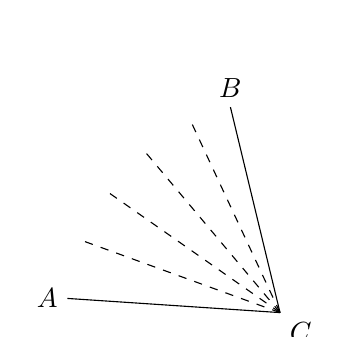
\begin{tikzpicture}[scale=0.9]
  \coordinate (C) at (0,0);
  \coordinate (A) at (-3,0.2);
  \coordinate (B) at (-0.7,2.9);
  \draw (C)--(A);
  \draw (C)--(B);
  \foreach \ang in {115,130,145,160} {\draw[dashed] (C)-- ++(\ang:3);}
  \node[left] at (A) {$A$};
  \node[above] at (B) {$B$};
  \node[below right] at (C) {$C$};
\end{tikzpicture}
\end{center}
% ---- printed p.23 (PDF 28) ----
Uendelige bliver altsaa baade som det uendelig Store og det uendelig Lille
omsluttet af endelige Grændser. Men, dersom det Uendelige virkelig omsluttes af
endelige Grændser, maa det jo dog, det siger den sunde Forstand, paa en eller
anden Maade selv være endeligt.

Hvordan hænger dette nu egentlig sammen? Som veiledende Exempler kunne vi engang
betragte de trigonometriske Functioner.
\[
AB = f_1(x) = \sin x;\quad BC = f_2(x) = \cos x;\quad
DF = f_3(x) = \operatorname{tg} x,\quad EG = f_4(x) = \cot x \ \text{o.\ s.\ v.}
\]

% FIGURE (printed p.23): unit circle, centre C; horizontal radius CD, vertical
%   radius CE; radius CA at angle x extended through F (on the vertical tangent
%   at D) to G (on the horizontal tangent at E); B = foot of perpendicular from A.
%   AB = sin, CB = cos, DF = tg, EG = cot.
\begin{center}
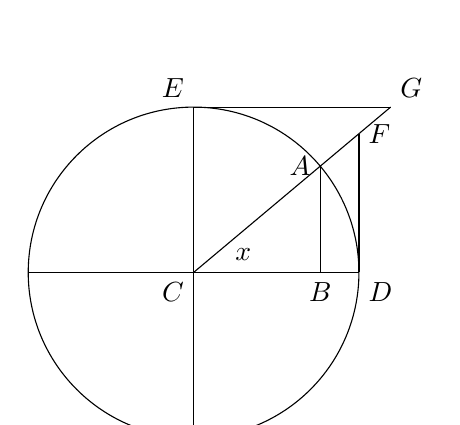
\begin{tikzpicture}[scale=2.1]
  \coordinate (C) at (0,0);
  \coordinate (D) at (1,0);
  \coordinate (E) at (0,1);
  \coordinate (A) at ({cos(40)},{sin(40)});
  \coordinate (B) at ({cos(40)},0);
  \coordinate (F) at (1,{tan(40)});
  \coordinate (G) at ({1/tan(40)},1);
  \draw (C) circle (1);
  \draw (-1,0)--(1,0);
  \draw (0,-1)--(0,1);
  \draw (C)--(G);
  \draw (A)--(B);
  \draw (D)--(F);
  \draw (E)--(G);
  \node at ({0.32*cos(20)},{0.32*sin(20)}) {$x$};
  \node[below left] at (C) {$C$};
  \node[below] at (B) {$B$};
  \node[below right] at (D) {$D$};
  \node[above left] at (E) {$E$};
  \node[left] at (A) {$A$};
  \node[right] at (F) {$F$};
  \node[above right] at (G) {$G$};
\end{tikzpicture}
\end{center}

Idet $x$, vor uafhængige Variable, voxer i første Quadrant, voxer, som bekjendt,
$\sin$, $\operatorname{tg}$, $\sec$ med det Samme, hvorimod $\cos$,
$\operatorname{cotg}$, $\operatorname{cosec}\ldots$ aftage. Forandringerne i $x$
gaae i første Quadrant fra $0^{\circ}$ til $90^{\circ}$; det er nødvendigt, at
betragte disse Forandringer nærmere.

Er $x = 0$, saa er $\sin x = 0$, men $\cos x = 1$; $\operatorname{tg} x = 0$, men
$\cot x = \infty$, $\sec x = 1$, men $\operatorname{cosec} x = \infty$; er
$x = 90^{\circ}$, da $\cos x = 0$, $\sin x = 1$, $\operatorname{tg} = \infty$,
$\cot x = 0$, o.\ s.\ v.

Det Endelige og det Uendelige bestemmes her ved hinanden saaledes, at Overgangen
fra Endeligt til Endeligt falder sammen med Overgangen fra Endeligt til
Uendeligt, hvorved da ogsaa en Overgang fra Endeligt til $0$ falder sammen med en
Overgang fra Endeligt til $\infty$.

Hvad betyder Udtrykket: $\angle x = 0$? I endelig Forstand kunde det betyde, at
her slet intet $x$ var; men i Kraft af Functionsbegrebet betyder $\angle x = 0$
et Ikke-Værende som dog er et Værende. At en Vinkel $= 0$ ingen Vinkel er,
forstaaer sig af sig selv; at $\angle x = 0$ dog alligevel betragtes som værende,
sees deraf, at Cosinus jo kun kan være en Vinkels Cosinus, og at $\cos 0$
ligesaavist er en reel Størrelse, som $\cos 1^{\circ}$.
% ---- printed p.24 (PDF 29) ----
% FIGURE (printed p.24): a detail of the circle — centre C, horizontal radius to
%   D, two close rays CA and CD' rising to the right, angle x = angle DCA.
\begin{center}
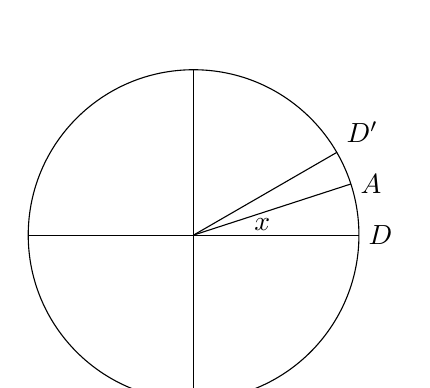
\begin{tikzpicture}[scale=2.1]
  \coordinate (C) at (0,0);
  \draw (C) circle (1);
  \draw (-1,0)--(1,0);
  \draw (0,-1)--(0,1);
  \coordinate (D) at (1,0);
  \coordinate (A) at ({cos(18)},{sin(18)});
  \coordinate (Dp) at ({cos(30)},{sin(30)});
  \draw (C)--(A);
  \draw (C)--(Dp);
  \node at ({0.42*cos(9)},{0.42*sin(9)}) {$x$};
  \node[right] at (D) {$D$};
  \node[right] at (A) {$A$};
  \node[above right] at (Dp) {$D'$};
\end{tikzpicture}
\end{center}

Antages $A$ at være i en Grads Afstand fra $D$ og $D'$, saa følger heraf, at
Veien fra $1^{\circ}$ til $0^{\circ}$ ikke er længere end Veien fra $1^{\circ}$
til $2^{\circ}$. $A$ kan komme $D$ saa nær, man vil, saalænge $A$ ikke falder
sammen med $D$, er $\angle x$ en endelig Størrelse; men i det Øieblik $A$ falder
sammen med $D$ bliver $\angle x = 0$. Saalænge $x$ endnu er endelig, er $\cot x$
ogsaa endelig; men i det Øieblik $x$ bliver $= 0$, bliver $\cot x = \infty$.

Afstanden fra Endeligt til $0$ og fra Endeligt til $\infty$ er altsaa her som en
Afstand fra det ene Endelighedspunkt til det andet. Ligger det ene
Endelighedspunkt det andet uendelig nær, da kan nu det Samme siges om $0$ og
Endeligt, om $\infty$ og Endeligt.

Vilde man, for at belyse Forholdet mellem Rækkerne og de trigonometriske Linier,
hente en Analogi fra Æsthetiken, maatte man vel sige: de trigonometriske
Functioner ere classiske, de uendelige Rækker romantiske.

At have det Uendelige omsluttet af det Endelige er jo classisk, at opfatte det
Uendelige som et for det Endelige Hiinsidigt, Uopnaaeligt, romantisk. Hvilken af
disse Synsmaader giver nu Mathematiken Medhold?

Forsaavidt Mathematiken er en exact Videnskab, skulde man vel mene, den holdt paa
det Classiske; men see vi paa dens Brug af Kategorier som: „Tilnærmelse, uendelig
Tilnærmelse“, skulde man næsten troe, den sværmede for det Romantiske.

Det er med denne Antydning naturligviis ikke Meningen, at ville indblande det
Æsthetiske i det Mathematiske, eller opklare videnskabelige Begreber ved
uvidenskabelige Analogier. Den flygtige Hentydning til det Æsthetiske skulde blot
tjene til at udhæve Forskjellen imellem den dobbelte
% ---- printed p.25 (PDF 30) ----
Maade, hvorpaa det Endeliges Forhold til det Uendelige bliver opfattet.

Hvad ligger der da i Begrebet: Tilnærmelse, uendelig Tilnærmelse?

Ved „uendelig Tilnærmelse“ kan man da for det Første ikke tænke paa Tilnærmelse
til et Opnaaeligt; thi det Opnaaelige udtrykker just, at Tilnærmelsen maa ende med
Maalets Opnaaelse, og altsaa i sit Væsen være endelig. Tilnærmelse til et
Opnaaeligt indeholder ingen Modsigelse; et Uopnaaeligt uden Tilnærmelse er heller
% ERRATA APPLIED (from the p.4 „Rettelse."): the print here (p.25, line 9) reads
%   „Tilnærmelse til et Uopnaaeligt indeholder ingen Modsigelse"; the errata
%   directs „læs: Tilnærmelse til et Opnaaeligt". Corrected above to „Opnaaeligt".
ikke nogen Modsigelse. Der er saaledes intet Modsigende i den Sætning, at
parallele Linier, hvor meget de end forlænges, aldrig ville skjære hinanden. Naar
Mathematiken undertiden bruger det Udtryk om parallele Linier, at de, forlængede
i det Uendelige, ville skjære hinanden: da kan man herved ikke egentlig tænke paa
nogen Tilnærmelse; det er en Umulighed, her fremstilles under Mulighedens Form.

En uendelig Tilnærmelse, Tilnærmelse til et Uopnaaeligt, synes derimod at
frembyde den haardeste af alle Modsigelser. Ved Tilnærmelse maa man jo dog i en
eller anden Forstand komme Maalet nærmere; men at komme Maalet nærmere maa dog vel
være det Samme som at komme Opnaaelsen nærmere; men fra Opnaaelsen af det
Uopnaaelige er man jo altid lige langt borte.

Ikke desto mindre hævder Mathematiken Begrebet af en uendelig Tilnærmelse, og
nedslaaer enhver Modsigelse ved uimodsigelige Beviser. Saaledes i Læren om
Asymptoterne.

% FIGURE (printed p.25): a hyperbola branch (solid) and its asymptote (dashed)
%   from A along the axis; ordinates at B and B' meet the curve at D, D' and the
%   asymptote at E, E'. AB = x; BD = y (to the curve); BE = y_1 (to the asymptote).
\begin{center}
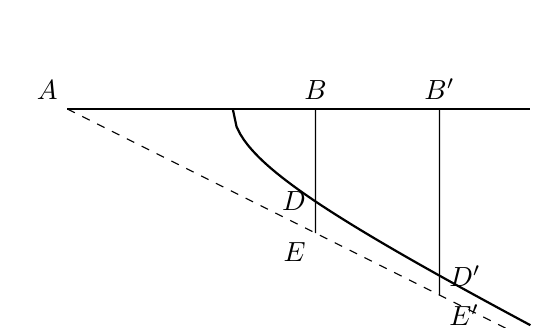
\begin{tikzpicture}[scale=1.05]
  \coordinate (A) at (0,0);
  \draw (A)--(5.6,0);
  \draw[dashed] (0,0)--(5.6,-2.8);
  \draw[thick] plot[domain=2:5.6,samples=80] (\x,{-0.5*sqrt(\x*\x-4)});
  \def\bx{3}\def\bpx{4.5}
  \coordinate (B) at (\bx,0);
  \coordinate (Bp) at (\bpx,0);
  \draw (B)--(\bx,{-0.5*\bx});
  \draw (Bp)--(\bpx,{-0.5*\bpx});
  \coordinate (D) at (\bx,{-0.5*sqrt(\bx*\bx-4)});
  \coordinate (E) at (\bx,{-0.5*\bx});
  \coordinate (Dp) at (\bpx,{-0.5*sqrt(\bpx*\bpx-4)});
  \coordinate (Ep) at (\bpx,{-0.5*\bpx});
  \node[above left] at (A) {$A$};
  \node[above] at (B) {$B$};
  \node[above] at (Bp) {$B'$};
  \node[left] at (D) {$D$};
  \node[below left] at (E) {$E$};
  \node[right] at (Dp) {$D'$};
  \node[below right] at (Ep) {$E'$};
\end{tikzpicture}

$AB = x;\quad BD = y;\quad BE = y_1.$
\end{center}

For Hyperblen har man f.\ Ex. Ligningen:
\[
f(x) = y = \frac{b}{a}\sqrt{x^{2} - a^{2}};
\]
for Hyperblens Asymptote:
% ---- printed p.26 (PDF 31) ----
$f_1(x) = y_1 = \dfrac{b}{a}x$. Altsaa er
\[
\begin{aligned}
y_1 - y &= \frac{b}{a}\left(x - \sqrt{x^{2}-a^{2}}\right)
= \frac{b}{a}\cdot
   \frac{\left(x-\sqrt{x^{2}-a^{2}}\right)\left(x+\sqrt{x^{2}-a^{2}}\right)}
        {x+\sqrt{x^{2}-a^{2}}}\\
&= \frac{b}{a}\cdot\frac{a^{2}}{x+\sqrt{x^{2}-a^{2}}}.
\end{aligned}
\]
Betragtningen af denne Formel viser, 1) at her er en virkelig Tilnærmelse, thi
jo større $x$ bliver, desto mindre bliver naturligviis Brøken
$\dfrac{a^{2}}{x+\sqrt{x^{2}-a^{2}}}$; 2) at Tilnærmelsens Maal er absolut
uopnaaeligt, thi Brøken er først $0$, naar $x$ er blevet $= \infty$.

Hvilken Gyldighed tør vi da tillægge Begrebet Tilnærmelse?

\begin{center}
  {\bfseries 2)\quad Rækker med stigende Potenser.}
\end{center}
\addcontentsline{toc}{subsection}{2) Rækker med stigende Potenser}

Skulle Begreberne: „Uopnaaeligt“, og „Tilnærmelse“ bringes i logisk Forbindelse,
da kunde man, ifølge „\textit{diversus respectus}“ maaskee begynde med at tænke
sig Sagen saaledes: Kategorien: „Tilnærmelse“ maa altid sees fra to Synspunkter:
1) det Punkt, hvorfra man gaaer ud, Begyndelsespunktet, og 2) det Punkt, der skal
naaes, Maalet, Endepunktet.

Gives der overhovedet nogen Bevægelse fra et bestemt Udgangspunkt henimod et
Maal, saa kan man, dersom Maalet er uendelig langt borte, jo i en Forstand gjerne
indrømme, at enhver Tilnærmelse er som et Intet imod Maalets uendelige Fjernhed,
og dog, naar man seer tilbage, betragte den fortsatte Fjernelse fra
Udgangspunktet som en Tilnærmelse til Maalet. Her er altsaa i en Henseende,
forsaavidt man nemlig seer fremad, ingen Tilnærmelse, men dog i en anden
Henseende, naar man vel at mærke seer tilbage, en virkelig Tilnærmelse.

Dialektiken kunde nu vistnok i denne Sammenhæng meget let confundere
„\textit{diversus respectus}“, og aflokke den
% ---- printed p.27 (PDF 32) ----
formelle Logik den Tilstaaelse, at den, ifølge egen Forklaring, altsaa dog kun
seer Tilnærmelsen som --- Bortfjernelse, kun seer fremad, forsaavidt den seer
tilbage, og at just dette er en Modsigelse; men vi have stillet os for
Mathematikens Forum, og tør ikke foregribe dens Kjendelse.

Forandringernes uudtømmelige Mulighed, der ligger skjult i Functionsbegrebet, som
i sin Grund, træder ved den intellectuelle Handling ud af denne Grund, og bliver
saa, under givne Betingelser, udviklet i de uendelige Rækker.

Skal en Function af $x$ indenfor Endelighedens Grændser udvikles i Række efter
Potenser, falder det naturligt, at begynde med den høieste Potens;
\[
\begin{aligned}
f(x) &= x^{n} + A_1 x^{n-1} + A_2 x^{n-2} + A_3 x^{n-3} + \dots A_{n-1}x + A_n\\
&= (x-a_1)(x-a_2)(x-a_3)\dots(x-a_n) = 0,
\end{aligned}
\]
en Række med faldende Potenser, er da et Paradigme.

Men, naar Opgaven er, at vise, hvorledes det Endelige i uendelig Tilnærmelse
stræber mod det Uendelige, maa Paradigmet ændres, og Functionen udvikles efter
stigende Potenser:
\[
f(x) = A_0 + A_1 x + A_2 x^{2} + A_3 x^{3} + \dots A_n x^{m} \dots
\]

Hvorledes nu en saadan Række kan fremstille den uendelige Tilnærmelse saavel til
$\infty$, som i sine enkelte Led, til $0$, er allerede klart af den geometriske
Progression.

I Rækken: $a\,\dfrac{1}{1-x} = a + ax + ax^{2} + \dots ax^{n-1}\dots$ bliver
$x^{\infty} = \infty$, dersom $x > 1$. Rækken vil da ikke blot kunne fortsættes
igjennem et uendeligt Antal Led, men med hvert følgende Led stedse komme $\infty$
nærmere. For $x < 1$ er $x^{\infty} = 0$. Rækken vil altsaa ved at fortsættes
gjennem utallige Led ikke alene give en større og større Sum, men hvert følgende
Led blive mindre og mindre, og altsaa nærme sig $0$.

Mathematiken kan ikke, som den formelle Logik, slaae sig til Ro ved en Forklaring
af „uendelig Tilnærmelse“ i
% ---- printed p.28 (PDF 33) ----
Ord; den bruger sit Tegnsprog, og articulerer Begrebet, idet den for enhver
uendelig Række udfinder Relationen imellem de enkelte Led.

For at dette kan skee, maa Functionsbegrebet antage en bestemt Charakteer: $f(x)$
f.\ Ex. $= a^{x}$. Man har da Rækken
$a^{x} = A_0 + A_1 x + A_2 x^{2} + A_3 x^{3} + \dots A_m x^{m} \dots$

For det mulige Tilfælde: $a^{x} = a^{0}$, er det let at bestemme Rækken
$a^{0} = A_0$; det Øvrige bortfalder. Men $a^{0} = A_0 = 1$. Da nu $f(x) = a^{x}$
skal, ifølge Functionsbegrebet, gjælde for alle mulige Værdier af $x$, har man i
denne Function første Coefficient $A_0 = 1$ een Gang for alle bestemt.

Cartesiusses Methode\footnote{C.\ Ramus. Algbr.\ F.\ S.\ 82. --- De ubestemte
Coefficienters Methode. Er $f(x) = A_0 + A_1 x + A_2 x^{2} + \dots
= B_0 + B_1 x + B_2 x^{2} + \dots$, saa maa $A_0$ være $= B_0$, $A_1 = B_1$,
$A_2 = B_2$ o.\ s.\ v. Beviis. For $x = 0$ bliver $A_0 = B_0$ alene tilbage; ved
at fradrage $A_0 = B_0$, faaer man $A_1 x + A_2 x^{2} = B_1 x + B_2 x^{2}\dots$,
ved at dividere med $x$, $A_1 + A_2 x\dots = B_1 + B_2 x$, og, ved at sætte
$x = 0$, $A_1 = B_1$ o.\ s.\ fr.} og Newtons Binomialformel\footnote{Binomial\-%
formlen. Fra den elementære Algebra kjender man: $(a+b)^{2} = a^{2} + 2ab +
b^{2}$; $(a+b)^{3} = a^{3} + 3a^{2}b + 3ab^{2} + b^{3}\dots$ o.\ s.\ v. Ram.\
Elmt.\ Algbr.\ S.\ 35. I den høiere Mathematik (Ramus Algebr.\ Functl.\ S.\ 85)
fremstilles $(p+x)^{n} = p^{n} + \frac{n}{1}p^{n-1}x + \frac{n(n-1)}{1\cdot 2}
p^{n-2}x^{2} + \frac{n(n-1)(n-2)}{1\cdot 2\cdot 3}p^{n-3}x^{3}\dots$, en Række
efter faldende Potenser af $p$ og stigende Potenser af $x$, hvis Coefficienter
dannes, som Analogien viser, paa en til Potensexponenterne svarende Maade.} give
derhos Mathematikeren Midler til, hvad de øvrige Led angaaer, at bringe det
Foranderlige til at gaae op i det Uforanderlige, og, saa at sige, fange de
uendelige Muligheder i Relationernes Net.
% [text to be added: pp. 29--... body batch 5]

\end{document}
